\documentclass{article}
\usepackage{icomp2026_conference,times}

\usepackage[T1]{fontenc}
\usepackage[utf8]{inputenc}
\usepackage[english]{babel}
\usepackage{hyperref}
\usepackage{url}
\usepackage{booktabs}
\usepackage{nicefrac}
\usepackage{microtype}
\usepackage{xcolor}
\usepackage{graphicx}
\usepackage{subcaption}
\usepackage{amsmath,amssymb,amsfonts}
\usepackage{amsthm}
\usepackage{float}

\newtheorem{proposition}{Proposition}
\newtheorem{criterion}{Criterion}

\usepackage[capitalize]{cleveref}
\crefname{section}{section}{sections}
\Crefname{section}{Section}{Sections}
\crefname{table}{table}{tables}
\Crefname{table}{Table}{Tables}

\title{Delay-Embedding Analysis of Neural Network Training Logs:\\
Preconditions, Negative Results, and Validated Driver Recovery}

\author{
  Nickolay Karlov\\
  MIPT\\
  Moscow, Russia\\
  \texttt{karlov.na@phystech.edu}\\
  \And
  Alexey Kravatskiy\\
  MIRIAI\\
  Moscow, Russia\\
  \texttt{kravatskii.a@miriai.org}\\
}

\icomparxivcopy   % named preprint: show the authors, without claiming publication

\begin{document}

\maketitle

\begin{abstract}
Empirical dynamic modelling promises to recover the structure of a high-dimensional
system from scalar observations, which makes it attractive for monitoring neural network
training from logs that consume negligible memory. This report establishes when that
promise is redeemable. The embedding theorems of Takens and Stark reconstruct a compact
invariant set that the trajectory revisits. We measure recurrence directly and find it
absent over a whole run, then test the weaker hypothesis that short windows are locally
stationary, logging every optimisation step to make that testable. The training loss does
recur locally, but the binding constraint is the number of independent observations, which
no logging rate changes: the correlation time is $163$ steps against a transition of
$1615$, so the entire transition affords ten independent samples whether rows are written
every step or every tenth. We then
report three candidate signals for the delayed generalisation phenomenon known as
grokking, each of which separates training runs convincingly and none of which survives a
controlled comparison: an intrinsic-dimension estimate that reproduces closed-form
constants of a straight line, a function-space velocity that tracks weight decay rather
than generalisation, and a shared-manifold coupling that tracks configuration rather than
the transition. Against these we set a positive result obtained in the regime where
Stark's theorem does apply. Convergent cross mapping recovers an externally injected
driver from a single one-dimensional loss log in seven of eight coupled runs across two
architectures, with no false positives among the control runs whose driver is logged but
never applied, and with a limitation for strictly periodic drivers that we characterise
quantitatively. Testing the reverse cross map, which the ground truth of these runs fixes
by construction, shows that the dominant direction is recovered in seven of eight coupled
runs while controls converge in neither direction, and also that unidirectionality is not
demonstrable when the driver acts on the loss without delay. Finally, a factorial study
separating the training split from the initialisation shows that the delay is itself a
broadly distributed random variable, with thirty runs of one configuration spanning $1290$
to $5600$ steps and a single run of the same configuration reaching $11\,790$.
\end{abstract}

\textbf{Keywords:} empirical dynamic modelling, delay embedding, surrogate data,
convergent cross mapping, grokking, training diagnostics.

\section{Introduction}\label{sec:intro}

A training run exposes very little of itself cheaply. Weights and activations are large
and expensive to store, whereas scalar logs such as the training loss, the validation
loss and the parameter norm cost almost nothing. If the geometry of the underlying
optimisation could be reconstructed from those scalars, monitoring would become
inexpensive and architecture independent. This is the premise of empirical dynamic
modelling, and it rests on the embedding theorems of Takens \citep{takens1981detecting}
and, for forced systems, of Stark \citep{stark1999delay, stark2003delay}.

The premise is attractive for grokking, the delayed generalisation reported by
\citet{power2022grokking}, where a scalar precursor of the transition would be valuable
and where the weight norm is an obvious candidate observable. We evaluate that candidate
and two others, establish where delay embedding is and is not licensed on training logs,
and report a positive result in the regime where it is.

The organising claim is the following. The embedding theorems reconstruct a compact
invariant set that the trajectory revisits. A training run driven by an external signal
with its own attractor satisfies this requirement by construction. The intrinsic
optimisation transient does not. Results that respect this boundary reproduce across
architectures and controls; results that cross it recover artefacts of trajectory
smoothness or of run configuration. \Cref{sec:protocol} states the requirements every
claim in this report is held to. \Cref{sec:preconditions} then measures the precondition,
\cref{sec:negative} reports three signals that violate it, \cref{sec:ccm} reports the
positive result obtained inside it, and \cref{sec:phenomenon} measures how variable the
transition itself is.

\section{Validation requirements}\label{sec:protocol}

Delay-embedding statistics return a finite number on data satisfying none of the hypotheses
behind them, and three of the estimators used below proved circular, mis-specified or
underpowered in exactly that way. We fix the following requirements in advance and hold
every claim here to them. Each costs well under an hour of computation.

\begin{enumerate}
\item \textbf{Measure the precondition before invoking a theorem.} If the trajectory does
not revisit its past states, the language of attractors does not apply whatever an
estimator returns. \Cref{sec:preconditions} finds the precondition unmet over a whole run,
and \cref{sec:sampling} finds it met locally for one observable of the three.

\item \textbf{Calibrate on a system with a known answer, against a reference matched in
length and in sampling density.} A Lorenz attractor grows by $1.66$ across the embedding
range at $n = 12\,000$ and by $8.86$ at $n = 2000$, so a reference of the wrong length
manufactures a separation by itself (\cref{fig:dimension}b). At $dt = 0.01$ the same
attractor fails a determinism test at $p = 0.400$ and only at $dt = 0.1$ passes at
$p = 0.010$. A negative result means nothing unless a matched reference is positive.

\item \textbf{Justify preprocessing per series.} Subtracting a moving average manufactures
structure in a sparse series, and differencing removes the slow drivers one may be looking
for: the periodic drivers of \cref{sec:ccm} cross map at $0.09$ and $0.12$ differenced and
at $0.81$ and $0.80$ raw.

\item \textbf{Test against surrogates, with an ensemble large enough to express the
threshold.} A statistic that does not exceed an amplitude-adjusted Fourier ensemble reports
the linear autocorrelation of the series. With $39$ surrogates the smallest attainable rank
p-value, $1/40 = 0.025$, coincides with the Bonferroni threshold for two nulls and leaves
no room for the correction; we use $199$. Neither null has power in the strictly periodic
case (\cref{sec:periodic}).

\item \textbf{Include a control differing in one respect only.} The ghost drivers of
\cref{sec:ccm} are the model: identical architecture, schedule, loss trajectory and
logging, differing only in whether the coupling exists. Controls differing in several
respects at once cannot discriminate, which is how each signal of \cref{sec:negative} came
to look convincing.

\item \textbf{For a causal claim, test the reverse direction.} A cross map in one direction
establishes coupling, not causation. Run both at a matched embedding and read direction
from convergence, not skill, which \cref{sec:direction} shows reaches $0.57$ in the false
direction.

\item \textbf{Hold configuration fixed, vary only seeds, and record the expected sign in
advance.} A predictor of the transition must correlate with the delay across runs of one
configuration. This test falsified the most promising candidate in \cref{sec:negative}.
\end{enumerate}

\section{Preconditions for delay embedding}\label{sec:preconditions}

Takens' theorem and its extensions guarantee that a delay map is an embedding of an
\emph{invariant set}. The guarantee is asymptotic and geometric: the orbit must return
near its past states, so that neighbours in the reconstructed space are dynamically
related rather than merely adjacent in time. When this fails, nearest-neighbour
statistics measure the local tangent to the trajectory instead of the geometry of an
attractor, a distortion first identified by \citet{theiler1986spurious}.

We therefore measure recurrence before invoking any theorem. For a delay-embedded series
we fix a neighbourhood radius once, as a low quantile of all pairwise distances, and
report the recurrence rate as a function of a temporal exclusion window. Fixing the radius
once is essential; recomputing it after each exclusion would force the recurrence rate to
equal the quantile for any input whatsoever, an error we made and corrected during this
work. The shape of the resulting profile separates the two cases of interest. On an
invariant set the rate falls to a positive plateau, because genuine returns occur at all
temporal separations beyond the orbit's period. On a transient the rate decays towards
zero, because every close pair was adjacent in time.

The estimator is calibrated on systems with known answers. A Lorenz-63 trajectory retains
$0.93$ of its recurrence rate at the widest exclusion, whereas a monotone ramp, which has
no dynamics at all, decays to exactly $0.00$. \Cref{fig:preconditions} applies it to the
training logs.

\begin{figure}[H]
\centering
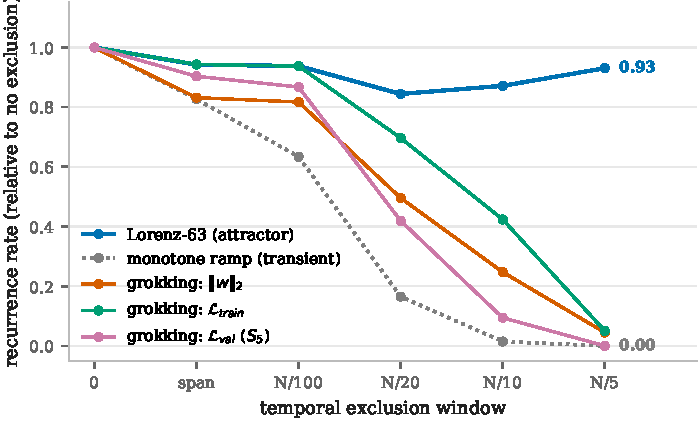
\includegraphics[width=0.72\textwidth]{figures/fig_preconditions.pdf}
\caption{Recurrence rate as a function of the temporal exclusion window, normalised by the
rate at zero exclusion. The Lorenz attractor holds a plateau, while all three training
observables decay towards the monotone-ramp reference. Over a whole run the trajectories
do not revisit their past states, so no single invariant set is available for the embedding
theorems to reconstruct. \Cref{sec:sampling} examines whether shorter windows escape this,
and finds that the training loss does recur locally while the weight norm does not.}
\label{fig:preconditions}
\end{figure}

All three training observables behave like the transient reference rather than like the
attractor. The validation loss of the $S_5$ runs reaches a ratio of $0.000$ and the weight
norm falls between $0.00$ and $0.07$.

That measurement is about the run as a whole, and by itself it settles less than it
appears to. Failing to return to its past states over twenty thousand steps does not
prevent a trajectory from being usefully stationary over a few hundred, and delay
embedding applied inside such a window would be legitimate. The global measurement rules
out treating a run as one invariant set; it does not rule out a local analysis. We
therefore test the local hypothesis directly.

\subsection{The sampling interval, and what it can and cannot fix}\label{sec:sampling}

A local analysis has two requirements that pull against each other: the window must be
short enough that the dynamics do not drift across it, and long enough to contain
independent observations. At one row per ten optimisation steps these cannot both be met.
A $300$-sample window, the length at which the dimension estimate of \cref{sec:dimension}
is computed, spans $3000$ optimisation steps against a median memorisation-to-generalisation
gap of $2875$: the window is longer than the transition it is meant to resolve.

We therefore re-ran three conditions logging every optimisation step. Only the inexpensive
series need that rate, since the training loss is already computed by the update and the
parameter norm is a reduction over the weights, whereas a validation pass is a forward pass
over the held-out split; the two are logged on separate schedules, and a test asserts that
neither the logging rate nor a skipped evaluation perturbs training.

\begin{figure}[H]
\centering
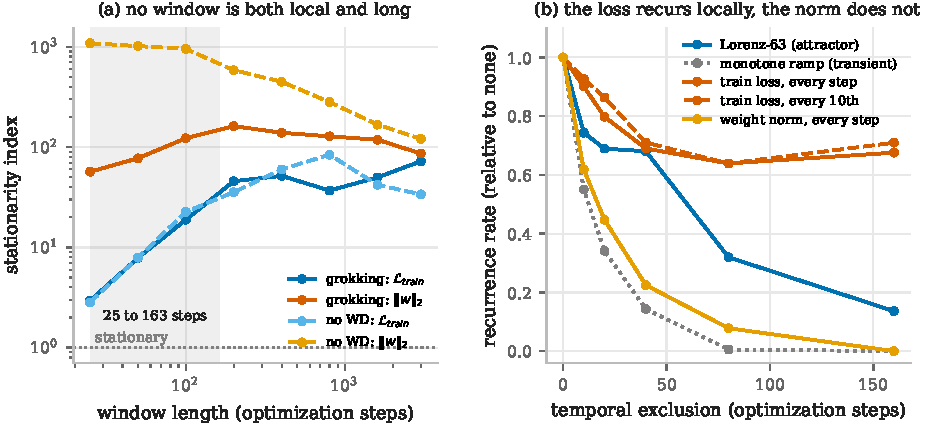
\includegraphics[width=0.95\textwidth]{figures/fig_local_stationarity.pdf}
\caption{(a) Stationarity index against window length, in units of the value white noise of
the same length produces, so unity means indistinguishable from stationary. The
normalisation is necessary: the unnormalised ratio falls as $1/\sqrt{L}$ for a stationary
series, so a fixed threshold would report long windows as more stationary by arithmetic
alone. The shaded band runs from the longest stationary window, $25$ steps, to one
correlation time of the training loss, $163$ steps. (b) Recurrence inside an $800$-step
segment against temporal exclusion. The training loss plateaus near the Lorenz reference
while the weight norm decays to the ramp, and logging ten times more densely leaves both
unchanged.}
\label{fig:localstat}
\end{figure}

Three results follow. First, and correcting the impression left by
\cref{fig:preconditions}, \emph{the training loss does recur locally}: inside an $800$-step
segment its profile plateaus between $0.64$ and $0.69$ against a Lorenz reference of
$0.68$, while the monotone ramp decays to $0.00$. The claim that training logs never
revisit past states holds globally and fails locally. Second, \emph{the weight norm does
neither}, decaying like the ramp and never falling below a stationarity index of $20$ at
any window length, against $1$ for a stationary series. Third, \emph{density was not what was missing}: the dense and decimated
profiles in \cref{fig:localstat}(b) agree throughout.

What binds is the number of independent observations, which is the window length divided by
the correlation time and so depends on neither the logging rate nor our choices. Inside the
transition the training loss has a correlation time of $163$ steps against a gap of
$1615$, giving ten independent samples whether a row is written every step ($1615$ rows) or
every tenth ($161$ rows). Against this, \cref{fig:dimension}(b) puts the length needed to
resolve even a Lorenz attractor at $n \gtrsim 6000$. The two constraints close from both
sides: the longest window indistinguishable from stationary is $25$ steps, shorter than a
single correlation time, so no scale is both stationary and observed more than once
independently.

The autocorrelation agrees. The dense training loss falls to $0.76$ at lag one and is then
flat near $0.72$, an independent minibatch-sampling term of about a quarter of the variance
on a slowly varying component, rather than dynamics hidden below the previous resolution;
a Lorenz trajectory at comparable density instead decays smoothly through $0.87$, $0.61$,
$0.38$, $0.23$. Consistent with this, no training observable exceeds an IAAFT surrogate
ensemble under simplex projection, the grokking training loss scoring $0.739$ against a
surrogate mean of $0.722$ at $p = 0.52$. That comparison is only interpretable against a
reference at comparable density, as \cref{sec:protocol} requires: Lorenz at $dt = 0.01$ is
oversampled in the same way and also fails, at $p = 0.400$, while at $dt = 0.1$ it passes
at $p = 0.010$.

One caveat constrains recurrence as a diagnostic. Independent noise also produces close
pairs at arbitrary separations and scores near unity, so recurrence separates smooth
transients from everything else but not an attractor from noise, which is why the
determinism test above accompanies it.

\section{Signals that do not survive controlled comparison}\label{sec:negative}

\subsection{Intrinsic dimension of the weight-norm trajectory}\label{sec:dimension}

The Levina--Bickel maximum likelihood estimator \citep{levina2004maximum} applied to a
sliding window of the weight-norm series produces a curve that rises during memorisation
and falls before generalisation. Four observations remove its interpretation as a
dimension. The first is analytic.

\begin{proposition}[The estimate is a constant of a straight line]\label{prop:line}
Let the delay vectors be sampled at uniform intervals from a curve that is locally
straight at the scale of the neighbourhood, and let a Theiler exclusion of $W$ samples be
applied. The $k$ nearest neighbours of an interior delay vector are then its temporal
neighbours at offsets $\pm(W{+}1), \pm(W{+}2), \dots$, so the ordered neighbour distances
satisfy $r_j \propto s_j$, where $s$ is the non-decreasing sequence
$W{+}1, W{+}1, W{+}2, W{+}2, \dots$ truncated to $k$ terms. The Levina--Bickel estimate
\begin{equation}\label{eq:lb}
  \hat{d} \;=\; \Bigl[\tfrac{1}{k-1}\textstyle\sum_{j=1}^{k-1} \log (r_k / r_j)\Bigr]^{-1}
  \;=\; (k-1) \Bigl/ \textstyle\sum_{j=1}^{k-1} \log (s_k / s_j)
\end{equation}
is therefore a function of $k$ and $W$ alone, and contains no information about the data.
For $k = 5$ it equals $1.330$ when $W = 0$ and $10.765$ when $W = 14$.
\end{proposition}

\Cref{fig:dimension}(a) verifies this. On a synthetic straight line the estimator returns
the predicted constant to within $1.1\%$ at every $k$ and $W$ tested, and on the two
control runs trained without weight decay, which never generalise, it returns the same
constants: medians of $1.33$ and $1.38$ without exclusion against a prediction of $1.33$,
and $11.30$ and $11.69$ with exclusion against $10.76$. Both plateaus are reproduced by a
straight line.

\begin{figure}[H]
\centering
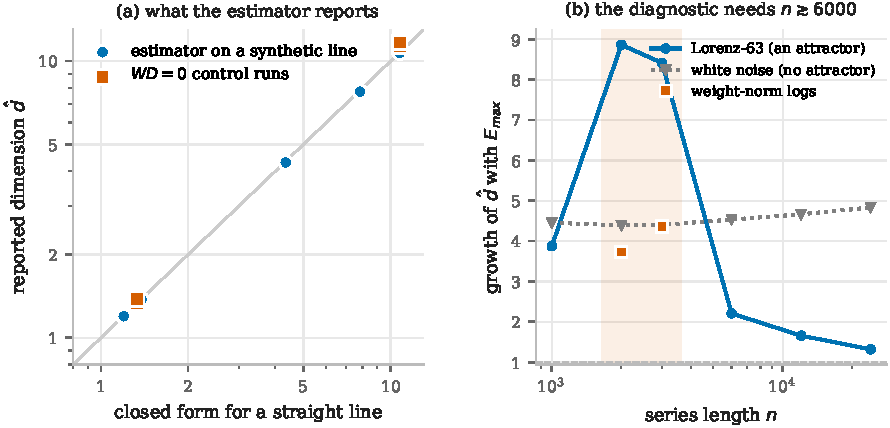
\includegraphics[width=0.95\textwidth]{figures/fig_dimension_artifact.pdf}
\caption{(a) Dimension reported by the estimator against the closed form of
\cref{prop:line}, on logarithmic axes with the identity line shown. (b) Growth of the
estimate between $E_{max} = 5$ and $E_{max} = 30$, against series length. A value near
unity is the signature of a resolvable attractor; the Lorenz reference reaches it only
beyond $n \approx 6000$, and inside the shaded band, the length training logs provide, it
scores worse than both white noise and the logs.}
\label{fig:dimension}
\end{figure}

The second observation is that no dimension is identifiable at this sample size. An
intrinsic dimension exists only if the estimate is insensitive to the space it is measured
in, but that diagnostic is itself strongly length-dependent: a Lorenz reference grows by
$8.86$ at $n = 2000$, $2.21$ at $n = 6000$ and $1.32$ at $n = 24\,000$, while white noise
holds between $4.4$ and $4.8$ (\cref{fig:dimension}b). At the lengths available it
therefore has no power, since a textbook attractor scores worse than the weight-norm series
it should outperform, at $8.86$ against $3.73$ and $4.36$. We draw no conclusion about
whether these logs resemble noise; what follows is a bound on the data budget, and
\cref{sec:protocol} states it as such.

The third observation is a controlled comparison, and it does not depend on a Theiler
exclusion, which the estimate is often computed without. \Cref{prop:line} at $W = 0$
returns $1.330$, so switching the exclusion off does not restore information; it pins the
estimate to the tangent constant, which is why such curves look stable. That disposes of
the reported \emph{level} but not of the \emph{shape}, since a control whose norm never
leaves a straight line is flat by construction and cannot refute a claim about a rise and a
fall. The control that can holds weight decay at $1.0$ and reduces the training fraction,
so the same regulariser drives a non-stationary norm in a model that never generalises.
\Cref{fig:papersettings} reports that comparison with no temporal exclusion at all.

The shape fails an internal check before reaching any control. Across three seeds of the
identical configuration, whose weight norms end at $29.89$, $29.12$ and $30.39$, the
estimate falls in one run (Spearman trend $-0.54$) and rises in the other two ($+0.94$,
$+0.90$), and their late-training levels are $1.51$, $9.21$ and $11.64$, a spread of $7.7$
within one configuration. The matched controls give $+0.75$ and $+0.22$, inside the range
spanned by the runs that generalise.

What the estimate tracks is local smoothness. Pooled over $1026$ windows it correlates at
Spearman $+0.887$ with $\mathrm{std}(\Delta x) / \mathrm{std}(x)$, computed without any
embedding, neighbour search or likelihood (\cref{fig:papersettings}c); within runs the
correlation ranges from $+0.32$ to $+0.996$, so smoothness is a strong correlate rather
than a complete description. The sign of the drift is immaterial, as expected of a
smoothness statistic: the grokking norm falls from $42$ to $30$ and the lowdata norm rises
from $42$ to $61$, and both collapse the estimate.

\begin{figure}[H]
\centering
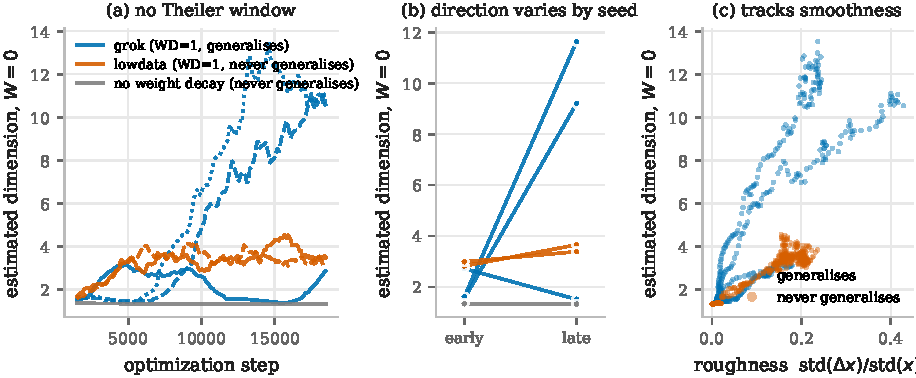
\includegraphics[width=0.99\textwidth]{figures/fig_paper_settings.pdf}
\caption{The dimension signal with no Theiler exclusion. (a) Sliding-window estimates; line
style distinguishes seeds. (b) Median estimate over the first and last third of training.
Two of three generalising runs rise, one falls, and the never-generalising runs lie between
them; the no-weight-decay run is flat at the tangent constant, its apparent decline
spanning only $1.34$ to $1.33$. (c) The estimate against a roughness ratio that involves no
embedding.}
\label{fig:papersettings}
\end{figure}

The fourth observation, from \cref{sec:sampling}, is that the weight norm is never locally
stationary at any window length from $25$ to $3000$ steps, with a stationarity index
between $20$ and $1087$. No window of it can be read as a stationary system, so the
estimate has no licensed interpretation even locally.

The third observation is procedural. The windows were labelled by their centres, so each
estimate incorporated data recorded after the step it was assigned to. Under causal
labelling, in which an estimate is assigned to the last step it observed, the reported
lead over the transition does not survive.

Averaging the per-point estimates also inflates them relative to pooling the likelihood,
as \citet{mackay2005comments} note. The correction changes the level but not the
conclusion, because the underlying quantity is not identifiable in the first place.

\subsection{Function-space velocity}

The preceding failure suggests an observable that cannot be a smoothness artefact of the
weight norm. We therefore recorded, at each logged step, the logits of a fixed probe set
of training inputs, centred each example's logit vector over classes and normalised it to
unit length. The resulting series is invariant to the uniform rescaling of logits that
weight decay induces, so a change in it indicates that the computed function has moved
rather than that its confidence scale has changed. The median per-example movement of the
normalised logits separates a grokking run from a run without weight decay by a factor of
approximately $360$.

The separation does not survive its control. We trained runs in which weight decay is held
at $1.0$ and only the quantity of training data is reduced, so that the model memorises
and never generalises. \Cref{fig:velocity} shows the outcome. The runs that never
generalise sustain a \emph{higher} velocity than the runs that grok. The comparison
carries three seeds of the grokking condition against four never-generalising runs, at two
training fractions with the smaller replicated across three seeds, and the two families do
not overlap. The only run far
below the others is the one without weight decay, in which the function freezes within a
few thousand steps and thereafter only rescales.

\begin{figure}[H]
\centering
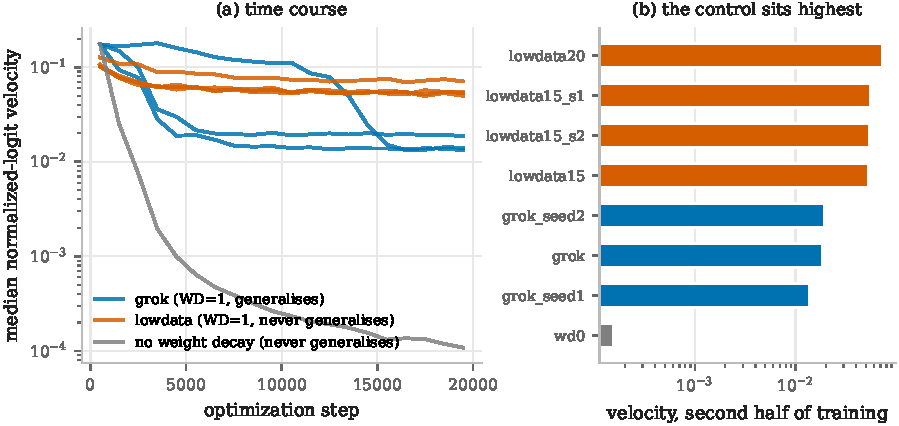
\includegraphics[width=0.95\textwidth]{figures/fig_velocity.pdf}
\caption{(a) Median velocity of the normalised probe logits against the optimization step,
on a logarithmic scale. (b) The same statistic over the second half of training, one bar
per run. If the velocity indicated impending generalisation, the runs that never
generalise would sit low. They sit highest. Weight decay is identical in the blue and
orange families, which differ only in the quantity of training data.}
\label{fig:velocity}
\end{figure}

Quantitatively, the runs that never generalise span $5.30\times10^{-2}$ to
$7.26\times10^{-2}$ over the second half of training against $1.38\times10^{-2}$ to
$1.94\times10^{-2}$ for the grokking runs, a separation of a factor of $2.73$ between the
closest members of the two families. The three seeds of the reduced-data condition agree to
within $3.4\%$, so the ordering does not rest on a single draw. The run without weight
decay falls to $1.53\times10^{-4}$. Every run with weight decay lies within a factor of five of every
other, and the factor of $360$ quoted above is entirely accounted for by the presence or
absence of regularisation. The statistic therefore measures the reorganisation that weight
decay imposes on the function, and among regularised runs it is, if anything, inversely
related to generalisation.

\subsection{Shared-manifold coupling}

Both preceding failures are statistics of a single transient series. Cross mapping asks a
different question, namely whether two observables lie on a common manifold, and that
question is well posed on a transient because it requires no recurrence of either series
alone. We therefore tested whether the training loss and the parameter norm, both
available without any validation data, share a manifold, and whether the coupling changes
at the transition.

The result appeared decisive. \Cref{fig:confound}(a) shows a clean separation with no
overlap: the three runs with a delayed transition have median coupling between $1.00$ and
$1.15$, while the four runs without lie between $2.87$ and $5.61$.

\begin{figure}[H]
\centering
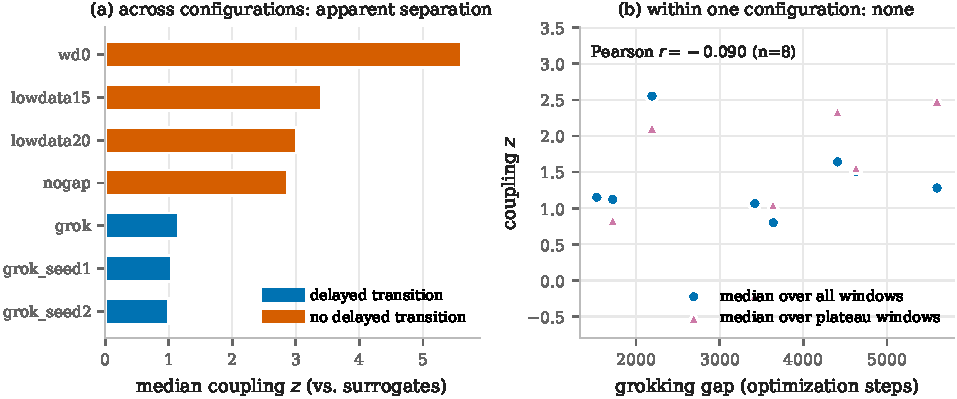
\includegraphics[width=0.92\textwidth]{figures/fig_confound_free.pdf}
\caption{(a) Median coupling between the training loss and the parameter norm separates
runs with a delayed transition from runs without. (b) The same statistic across eight runs
of a single configuration, in which only the split and initialisation seeds vary. The gap
spans $1290$ to $5600$ steps and the coupling is unrelated to it. The separation in panel
(a) reflects configuration, not the transition.}
\label{fig:confound}
\end{figure}

Two checks dissolve it. Within individual runs the statistic does not move at the moment
of generalisation; the apparent step in an aggregate over runs arises from averaging runs
whose transitions occur at different steps. More importantly, the grouping in panel (a)
coincides exactly with configuration, since the low group consists of the runs with a
training fraction of $0.3$ and weight decay of $1.0$ and the high group contains every
other setting. We therefore held configuration fixed and varied only the split and
initialisation seeds, which the study of \cref{sec:phenomenon} shows produce gaps between
$1290$ and $5600$ steps. The expected sign was recorded before the runs were executed.
The observed correlation between the gap and the coupling is $-0.090$ (Pearson) and
$+0.214$ (Spearman) over eight runs, that is, nothing, and for plateau windows it is
weakly positive, which is the opposite of the prediction. Within one configuration the
coupling spans $0.80$ to $2.55$, against $1.0$ to $5.6$ across configurations.

\subsection{A common failure mode}

The three fail in the same way, as \cref{tab:failures} summarises. Each separates
\emph{configurations} rather than \emph{transitions}, and each rests on a comparison in
which the runs differ in more than the property of interest. We regard this, rather than
any individual negative result, as the principal methodological lesson.

\begin{table}[H]
\centering
\caption{The three signals, the comparison that made each convincing, and the control that
falsifies it. In every case the falsifying control differs from the positive runs in one
respect only.}
\label{tab:failures}
\small
\begin{tabular}{@{}p{0.20\textwidth}p{0.24\textwidth}p{0.24\textwidth}p{0.22\textwidth}@{}}
\toprule
\textbf{Signal} & \textbf{Apparent evidence} & \textbf{Falsifying control} & \textbf{What it measures} \\
\midrule
Intrinsic dimension of $\lVert w \rVert_2$
& Rises then collapses before generalisation
& A straight line reproduces both plateaus; across seeds of one configuration the estimate rises twice and falls once
& Local smoothness of the series \\
\addlinespace
Function-space velocity
& Separates $WD=1$ from $WD=0$ by a factor of $360$
& $WD=1$ with reduced data never generalises, yet sustains a higher velocity
& Reorganisation imposed by weight decay \\
\addlinespace
Shared-manifold coupling
& Separates runs with a delayed transition from runs without, with no overlap
& Across eight runs of one configuration the coupling is unrelated to the delay, $r = -0.090$
& Run configuration \\
\bottomrule
\end{tabular}
\end{table}

\section{Driver recovery in the regime where the theorems apply}\label{sec:ccm}

Stark's extension of Takens' theorem covers a system driven by an external signal that
possesses its own attractor \citep{stark1999delay, stark2003delay}. A training run
modulated by an injected driver satisfies that hypothesis by construction, which makes it
the natural setting in which to ask whether anything at all is recoverable from a
one-dimensional log.

\subsection{Design}

We use two independent settings. The first consists of existing logs from a ResNet-18
trained on CIFAR-10, in which a fraction of each batch's labels is corrupted according to
a driver logged alongside the loss. The second reproduces the design in this work, using a
one-layer transformer on modular addition with drivers under our control. In both cases
the ground truth is known, and in both cases the essential control is a \emph{ghost}
driver, which is logged exactly like a real one while the batch is returned unmodified.
A ghost run shares the architecture, the schedule, the loss trajectory and the logging
cadence of a coupled run and differs only in whether coupling exists.

Detection uses convergent cross mapping \citep{sugihara2012detecting}: the response is
delay embedded and used to predict the driver, on the reasoning that if the driver forces
the response then the reconstructed manifold of the response carries information about the
driver's state. Significance is assessed against two nulls. The first uses iterative
amplitude-adjusted Fourier surrogates \citep{theiler1992testing, schreiber1996improved},
which preserve the power spectrum and the exact value distribution of the driver while
destroying its alignment with the response. The second rotates the driver in time, which
preserves every value and changes only the alignment. No result is reported without them.

\subsection{Results}

\begin{figure}[H]
\centering
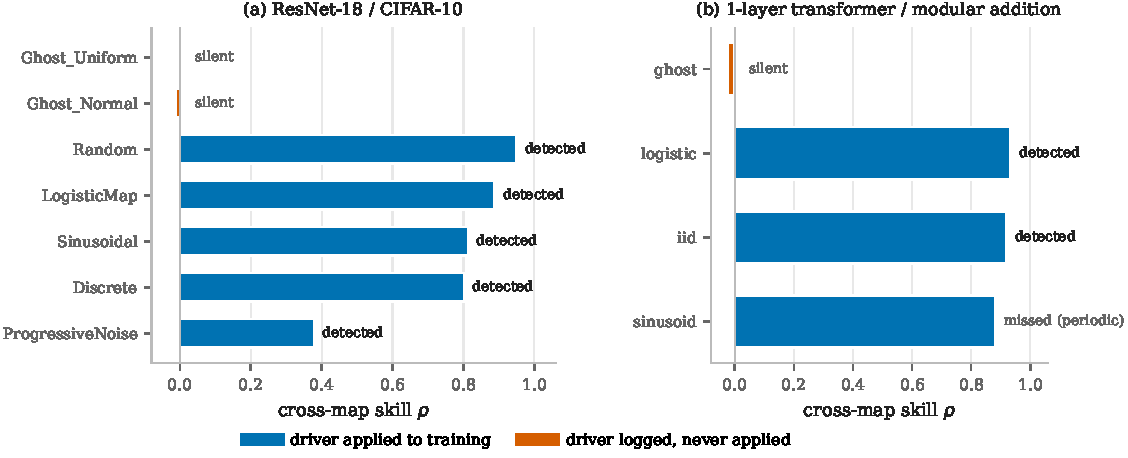
\includegraphics[width=0.95\textwidth]{figures/fig_driver_recovery.pdf}
\caption{Cross-map skill for every run in both settings. Drivers that were applied to
training are recovered from the loss log alone; drivers that were logged but never applied
are not. The single missed detection is the smooth periodic driver discussed in
\cref{sec:periodic}.}
\label{fig:recovery}
\end{figure}

\Cref{fig:recovery} summarises both settings. All five coupled drivers in the ResNet
setting are detected, with skills between $0.379$ and $0.949$ and $p \le 0.05$ under both
nulls; in the transformer setting the chaotic and independent drivers are detected at
$0.934$ and $0.919$. Seven of eight coupled runs are detected and no ghost produces a false
positive. Three of the five ghosts carry a varying driver and cross map at $-0.011$,
$-0.007$ and $-0.024$; the other two carry a constant driver with no variation to recover,
so they are controls but not evidence, and are omitted from \cref{fig:recovery}.

The ghosts carry the argument. They share the training trend with the coupled runs, so
their near-zero skill excludes the explanation that defeated every signal of
\cref{sec:negative}, that a statistic separates runs because their loss curves have
different shapes.

The rule declares a driver recovered when either null rejects, a family of two tests whose
false-positive rate approaches $0.10$ rather than $0.05$, and the $39$-surrogate ensemble
cannot express the correction because its p-value floor of $0.025$ is the Bonferroni
threshold itself. Repeating both experiments with $199$ surrogates leaves every verdict
unchanged: seven true positives, one false negative, no false positives under either rule.
The one marginal case, the ResNet periodic driver at $p = 0.050$, resolves to $p = 0.015$.

Convergence with library size, the signature that gives the method its name and
distinguishes causation from coincidental correlation, is shown for both directions in
\cref{fig:direction}(a): skill rises for the coupled runs, most clearly for the independent
driver at $0.59$ to $0.95$, while the ghosts show neither rise nor level. Differencing the
response, the obvious way to remove the training trend, inverts this conclusion by removing
the slow drivers with it (\cref{sec:protocol}); no manual removal is needed, since both
nulls and the ghosts already control for the trend.

\subsection{A limitation for periodic drivers}\label{sec:periodic}

The one missed detection is instructive and is not repaired by a better statistic. The
smooth sinusoidal driver of the transformer setting yields a cross-map skill of $0.882$,
which is high, but its surrogates reach between $0.87$ and $0.94$, which is equally high.
The reason is structural. The loss reveals the phase of the cycle, and any series of the
same period, whether a spectrum-preserving surrogate or the driver rotated in time, is a
deterministic function of that phase and is therefore equally predictable from it.
Spectrum-preserving nulls consequently have no power against a strictly periodic driver.
The corresponding driver in the ResNet setting is detected only because it is quantised to
ninety-five distinct values, so its surrogates depart from it considerably further. A
different null, for example a driver of a different period, would be required.

\subsection{Direction of the recovered coupling}\label{sec:direction}

Detection is not direction: recovering the driver from the loss shows the two are coupled,
not which forces which. Cross mapping is asymmetric and can be asked directly. Embedding
$Y$ and predicting $X$, written $Y$ xmap $X$, is evidence that $X$ drives $Y$
\citep{sugihara2012detecting}, so the forward map is loss xmap driver. Here the ground
truth is known rather than assumed, since the driver schedule is evaluated from a fixed
seed before any gradient is taken and cannot depend on training.

The convention is calibrated on a system with a known answer, as inverting it would invert
every causal statement resting on it. On coupled logistic maps with $\beta_{xy} = 0$ and
$\beta_{yx} = 0.32$, so $X$ drives $Y$ alone, the true direction rises from $0.331$ to
$0.993$ with library size while the false direction runs $0.585$ to $0.569$ and does not
converge. The false direction reaches a skill of $0.57$ while carrying no causal
information, which establishes that convergence rather than skill is the discriminating
quantity.

\begin{figure}[H]
\centering
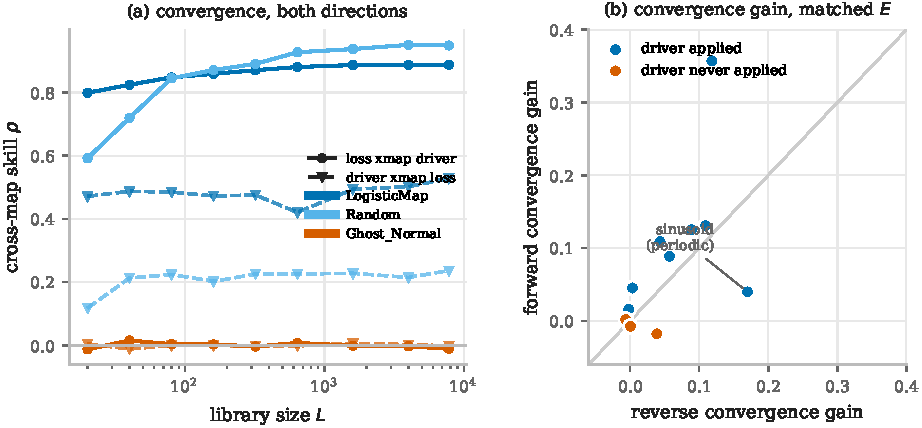
\includegraphics[width=0.95\textwidth]{figures/fig_directionality.pdf}
\caption{Forward against reverse cross mapping, both at a matched embedding dimension.
(a) Skill against library size: the forward map converges for coupled runs while the
reverse stays flat, and both are flat for the ghost. (b) Convergence gain. Coupled runs lie
above the diagonal and ghosts sit at the origin; the exception is the periodic driver of
\cref{sec:periodic}.}
\label{fig:direction}
\end{figure}

At a matched embedding the forward map converges more strongly than the reverse in seven of
eight coupled runs, most clearly for the independent driver at gains of $0.357$ against
$0.118$, while the ghosts converge in neither direction with all gains within $0.039$ of
zero. The exception is the periodic driver, whose reverse gain of $0.170$ exceeds its
forward $0.040$; that run also fails forward detection at $p = 0.77$ and is excluded by
\cref{sec:periodic} on independent grounds.

A stricter reading does not support unidirectionality. Granting the reverse the best of
five embedding dimensions rather than holding it at the forward's $E = 3$, it converges and
beats its own null in most runs: no coupled run is then read as unidirectional and five of
eight are read as bidirectional. Selecting a maximum over five embeddings inflates the
reverse, but not by itself. The explanation is structural: the driver acts at every step,
so the loss depends on it contemporaneously and a delay vector of the driver already
contains the value the loss is partly a function of, letting the reverse map succeed by
direct functional dependence with no manifold involved. Cross mapping does not separate
causation from strong instantaneous coupling, the generalised-synchrony regime
\citep{rulkov1995generalized} known to compromise it \citep{ye2015distinguishing}.

We therefore claim the dominant direction, recovered correctly in seven of eight runs, and
not unidirectionality. Establishing the latter would require a driver acting with a delay,
so that the contemporaneous term is absent.

\subsection{The method is not discriminative between a run's own metrics}

For completeness we applied the same procedure to pairs of observables within single
uninjected runs. Eleven of sixteen directed pairs pass both nulls, with skills as high as
$1.000$. This is consistent with the theory, since the training loss, the validation loss
and the parameter norm are three observations of one system, but it means that cross
mapping between a run's own metrics carries no information about the transition and should
not be interpreted as a discovery.

\section{Variability of the delayed transition}\label{sec:phenomenon}

Any statistic proposed as a precursor of grokking is a statement about the delay, so the
distribution of the delay is worth measuring before precursors are sought. The
configuration seeds a single random stream from which the train and validation split is
drawn and from which the model initialisation then continues. A change of seed therefore
alters both which examples are trained on and what the initial weights are, and the two
cannot be attributed separately. We separate them by restarting the stream between the two
steps, verify that the modification is inert when unused and that it decouples the two
factors in both directions, and run a factorial study of six splits by five
initialisations with weight decay fixed throughout.

\begin{figure}[H]
\centering
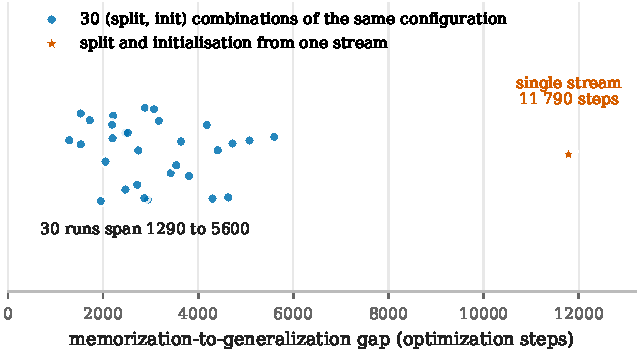
\includegraphics[width=0.72\textwidth]{figures/fig_delay_distribution.pdf}
\caption{Memorisation-to-generalisation gap for thirty runs of one configuration, varying
only the split and the initialisation seed. Every run generalises and every gap lies
between $1290$ and $5600$ steps. Marked separately is a run of the same configuration in
which the split and the initialisation are drawn from a single stream, whose gap of
$11\,790$ steps lies far outside the distribution.}
\label{fig:delays}
\end{figure}

All thirty runs generalise, with gaps between $1290$ and $5600$ steps, a mean of $3062$ and
a standard deviation of $1130$: within a configuration held otherwise fixed, the delay has
a standard deviation exceeding a third of its mean.

A run of the same configuration under the coupled stream produced a gap of $11\,790$ steps,
$7.7$ standard deviations above the grid mean and $2.11$ times its largest member, while
two further runs at other seeds gave $1510$ and $1570$, both inside it. Five grid cells
share the outlying run's split and give $2050$ to $4300$, so the split alone does not
account for it, and no cell reproduces the pairing of split and initialisation the coupled
stream produces; we attribute the outlier to that pairing. A delay measured from one run is
therefore not a property of the configuration, and a precursor validated against one run
has been validated against a single draw from a wide distribution.

The variance decomposition is inconclusive by design rather than by accident. The split
accounts for $19.8\%$ of the variance in the gap and the initialisation for $23.8\%$, with
the remainder in the interaction. Neither factor dominates. A partial analysis of the first
fifteen cells indicated the opposite, with the split accounting for $43\%$ against $17\%$
for the initialisation, which is a caution against reading factorial studies before they
complete.

\section{Conclusion}\label{sec:concl}

Delay-embedding methods apply to training logs in a narrower regime than their premise
suggests, and within it they work. When an external driver with its own attractor forces
training, convergent cross mapping recovers it from a single scalar loss log in seven of
eight coupled runs across two architectures, with no false positives among the runs whose
driver was logged but never applied, and the forward map converges more strongly than the
reverse in seven of eight. These data do not establish unidirectionality
(\cref{sec:direction}). The quantity needs no validation data and comes from a log that
costs nothing to store.

The intrinsic optimisation transient does not admit the same treatment, for a quantitative
reason rather than a matter of taste: its correlation time is a tenth of the transition it
would have to resolve, so the transition affords about ten independent observations at any
logging rate, against the thousands an attractor reconstruction needs. The three statistics
that appeared to detect the grokking transition separate run configurations instead, and
the phenomenon is more variable than one run can reveal, thirty runs of a single
configuration spanning $1290$ to $5600$ steps against $11\,790$ for a run of the same
configuration seeded from one stream.

One question is left open: whether any training-side observable distinguishes a run that
will generalise from one that will not, with configuration held fixed. None of the five
examined here does, comprising the parameter norm, the trajectory roughness, the intrinsic
dimension, the function-space velocity and the shared-manifold coupling. The driven regime
is where the theory applies and validation against a known answer is possible, and it is
where we would place further effort.

\bibliographystyle{icomp2026_conference}
\bibliography{references}

\end{document}
